\documentclass[11pt,a4paper]{ctexart}
\usepackage{geometry}
\geometry{left=2.54cm,right=2.54cm,top=3.18cm,bottom=3.18cm}
\usepackage{booktabs}
\usepackage{float}
\usepackage{amsmath}
\usepackage{graphicx}
\usepackage{enumitem}
\usepackage{xcolor}
\usepackage[colorlinks=true,linkcolor=blue,citecolor=blue]{hyperref}
\usepackage{caption}
\usepackage{url}    

% 使用 ctex 原生命令设置标题格式，避免宏包冲突
\ctexset{
  section = {
    format = \Large\bfseries,
    name = {,},
    number = \thesection,
    aftername = \hspace{1em}
  },
  subsection = {
    format = \large\bfseries,
    name = {,},
    number = \thesubsection,
    aftername = \hspace{1em}
  }
}

\title{\vspace{-2cm}\textbf{\huge 大语言模型推理范式研究}\\[0.5cm] \Large 基于多智能体控制流的复杂任务性能评估}
\author{231240045 杨俊炜}
\date{\today}

\begin{document}

\maketitle
\thispagestyle{empty}

\begin{abstract}
\noindent 本研究旨在探索大语言模型（LLM）通过外部认知架构提升复杂任务求解能力的内在机制。基于大语言模型API，我设计并实现了三种典型的智能体控制流（Agent Control Flow）：基础直接提示（DirectPromptAgent）、思考与行动结合范式（ReActAgent）以及自我反思架构（ReflexionAgent）。实验在不同难度的开源数据集（GSM8K与HotpotQA）上展开，测试模型底座为 Qwen-flash，并采用性能更优的 Qwen-plus 作为裁判模型（LLM-as-a-Judge）进行横向量化评分。实验不仅量化对比了各架构在任务成功率、交互轮数及耗时上的表现，还在工程实现上针对工具调用、结果正则提取及评估维度进行了深度优化。结果表明，ReAct范式在复杂计算与多跳检索任务中表现出显著的优势，有效激发了模型的深度推理能力；而目前的Reflexion架构在此类强事实性任务上存在“过度思考”且效率较低的瓶颈。
\end{abstract}

\vspace{1cm}

\section{引言}
随着大语言模型（Large Language Models, LLMs）的快速发展，单次生成的直接提示（Direct Prompting）在处理复杂数学推理、多跳信息检索以及长程规划等任务时常遭遇瓶颈，易产生事实幻觉或逻辑断链。为了打破模型内部权重的认知局限，构建赋予LLM外部工具调用与记忆管理能力的智能体（Agent）成为前沿趋势。

本研究聚焦于多智能体推理范式的对比分析，通过编写 \verb|agent.py| 及 \verb|evaluate.py|，实现了Direct Prompt、ReAct和Reflexion三种架构的控制流，并在多维度评估其在复杂任务中的激发效果。研究旨在通过量化数据回答一个核心问题：不同的外挂认知架构如何实质性地改变LLM的解题行为与最终效能。

\section{实验设计与实现优化}

\subsection{评估模型与测试集构建}
在模型选型上，兼顾成本与响应速度，实验采用 \textbf{Qwen-flash} 作为所有Agent的驱动底座（生成模型）；为了保证评估的客观性与细粒度区分，采用更高参数量级的 \textbf{Qwen-plus} 作为裁判模型（LLM-as-a-Judge）。

测试集方面，我从权威开源数据集中自动拉取并构建了50道测试题，形成了难度分层的评估基准：
\begin{itemize}[itemsep=2pt,parsep=0pt,topsep=2pt]
    \item \textbf{数学推理（agent\_killer难度）}：选取25道 \textbf{GSM8K} 数据集题目，主要考察复杂的数学逻辑与计算能力。
    \item \textbf{多跳搜索（too\_hard难度）}：选取25道 \textbf{HotpotQA} 数据集题目，主要考察跨文档的事实检索与拼接推理能力。
\end{itemize}

\subsection{智能体控制流架构}
基于面向对象编程，我设计了三种具有代表性的基类继承Agent：
\begin{enumerate}[itemsep=2pt,parsep=0pt,topsep=2pt]
    \item \textbf{DirectPromptAgent}：作为基线模型，直接向大模型发起询问，不提供任何外部工具，依赖其参数化记忆（Parametric Memory）作答。
    \item \textbf{ReActAgent}：实现了推理（Reasoning）与行动（Acting）的交替迭代。大模型通过生成 \verb|Thought| 与 \verb|Action| 决定下一步动作，可执行操作有数学计算、互联网搜索、python代码执行。
    \item \textbf{ReflexionAgent}：引入了自我反思（Self-reflection）机制。模型在生成初版答案后，由内置的评价提示词引导其对答案的准确性与完整性进行评估，并基于反思建议迭代修正答案。
\end{enumerate}

\begin{figure}[htbp]
    \centering
    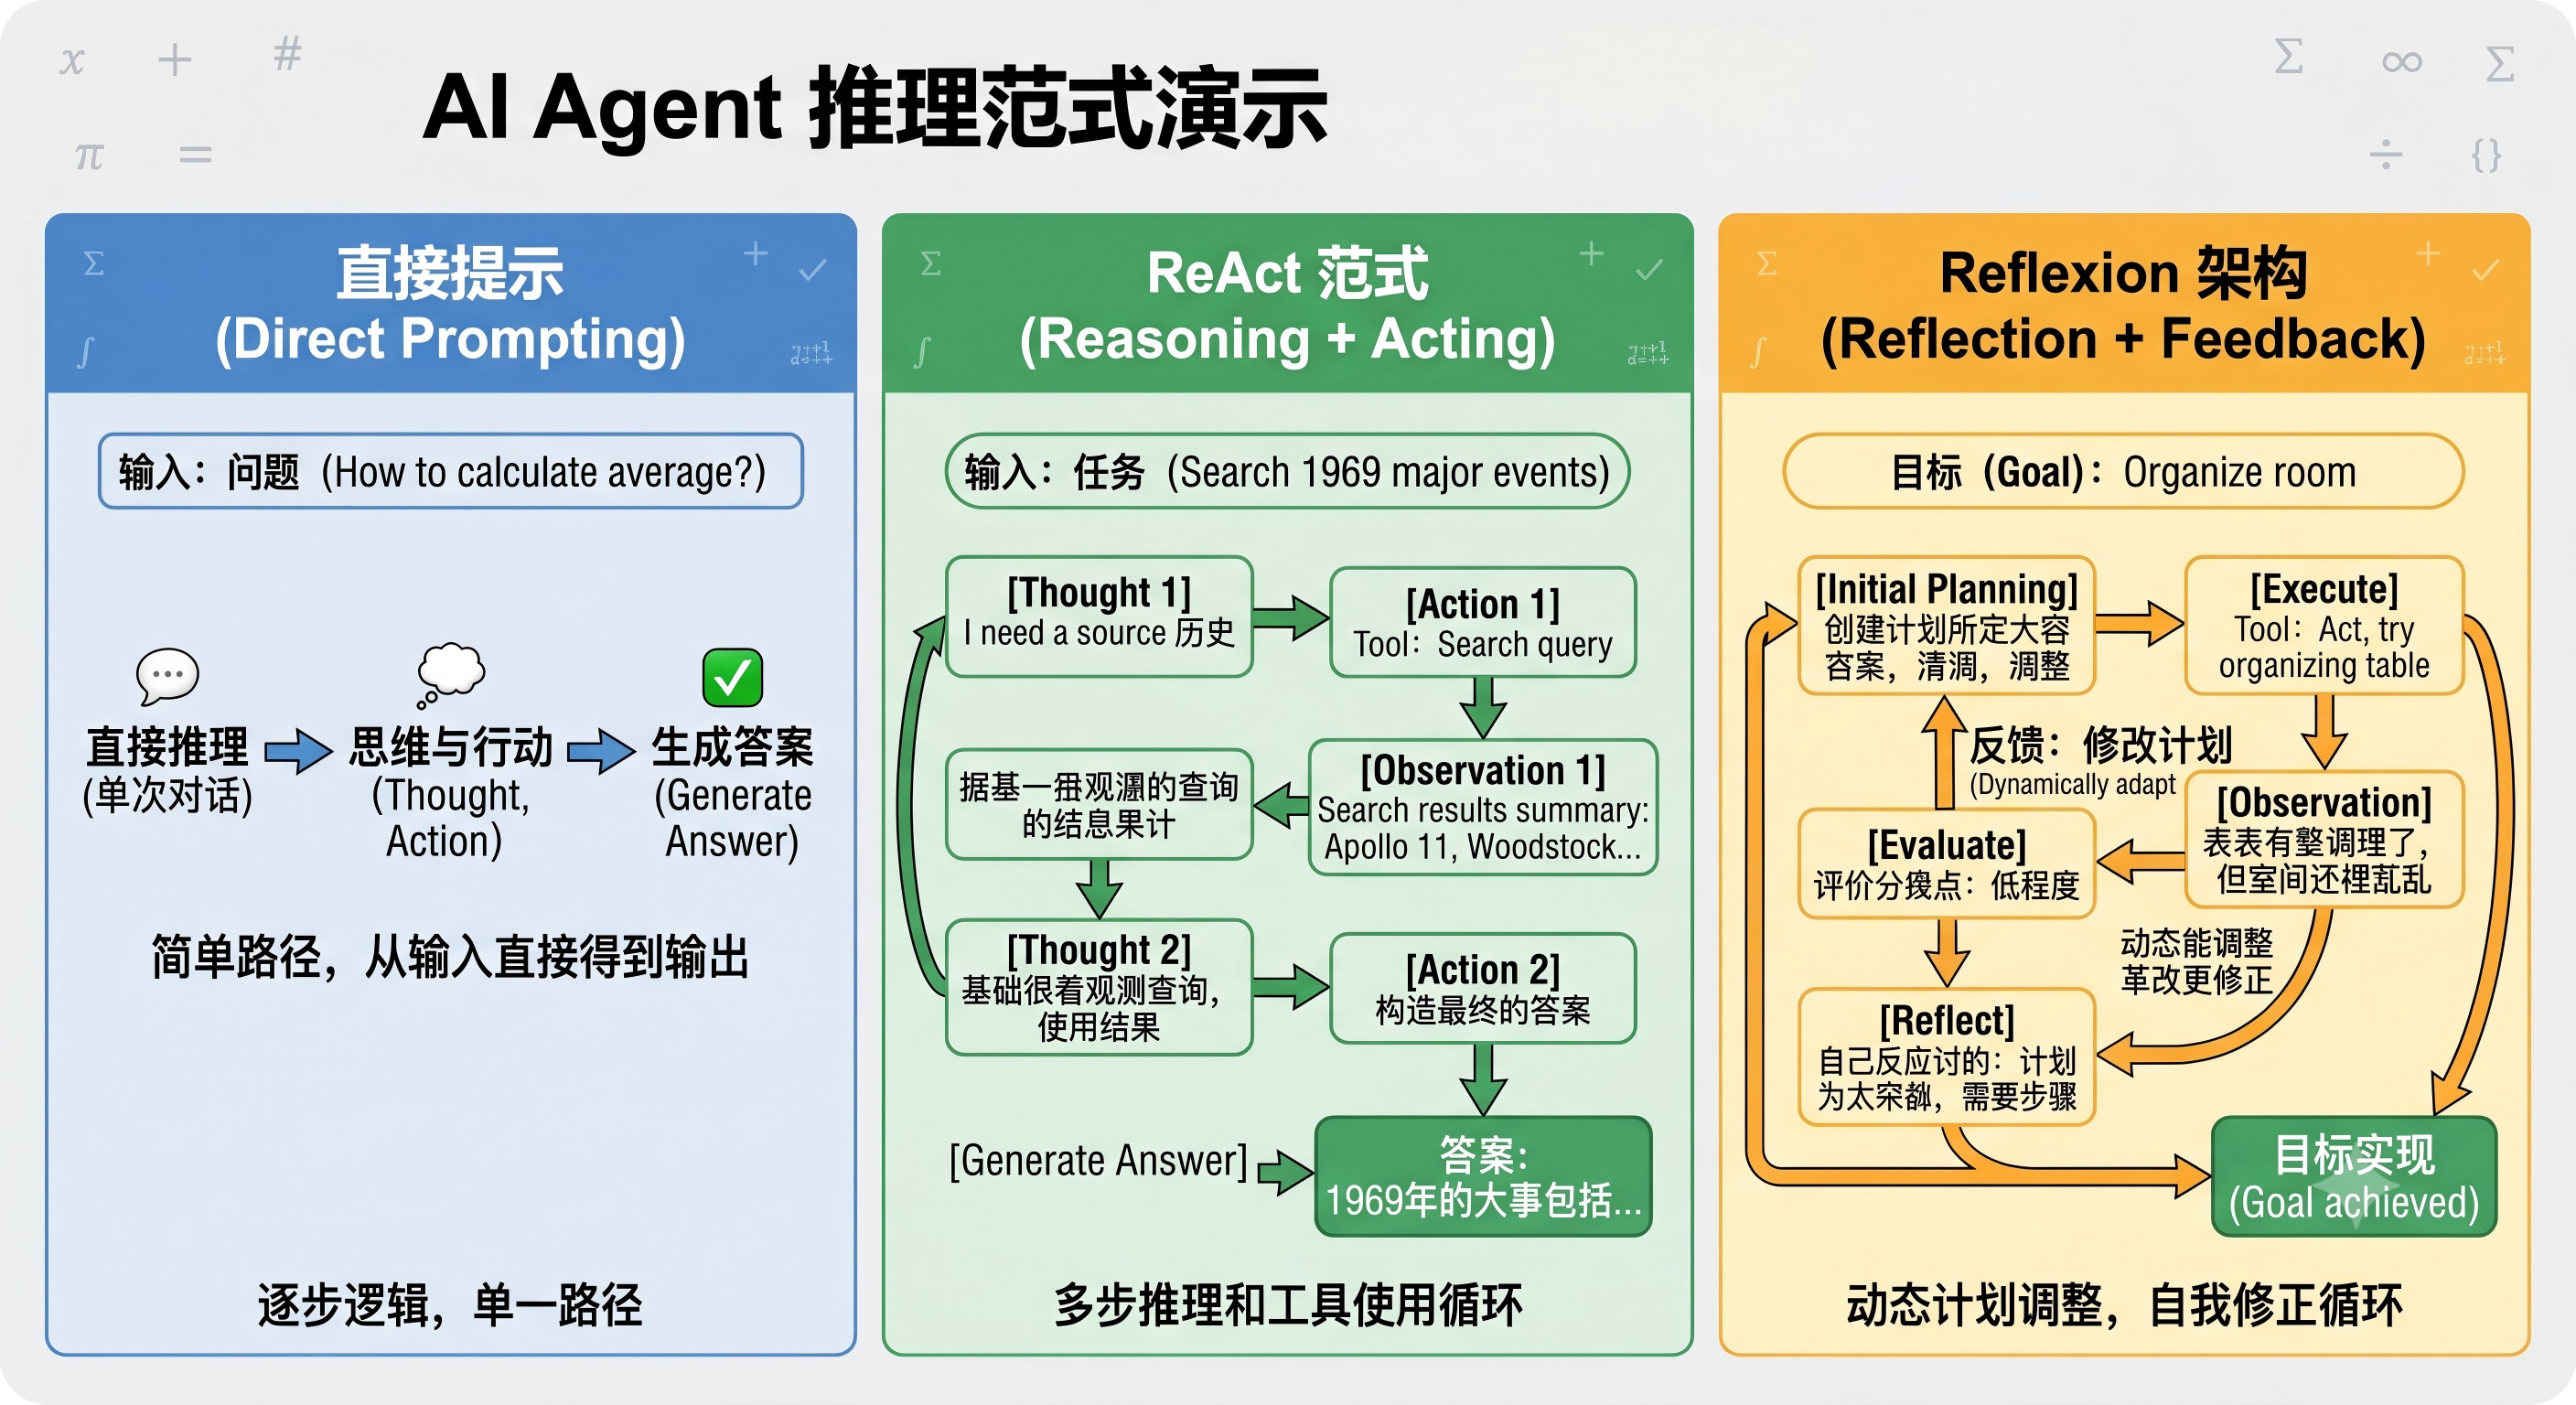
\includegraphics[width=0.9\textwidth]{agent架构.png}
    \caption{三种智能体控制流架构示意图}
    \label{fig:agent_architectures}
\end{figure}

\subsection{工程实践与深度优化}
在代码落地过程中，针对大模型在实际应用中暴露出的痛点，我实施了四项核心工程优化：

\paragraph{1. ReAct工具链的真实化升级：} 
从早期的本地字典模拟检索全面升级为真实环境的 API 调用。将 \verb|search| 工具桥接至 DuckDuckGo (DDGS) 进行互联网实时搜索，将 \verb|python| 工具实现为沙盒内的真实代码执行（限制 \verb|builtins| 并捕获标准输出）。这要求Agent具备处理真实世界复杂信息的过滤能力。

\paragraph{2. 结果提取策略的正则优化：}
在早期的测试中，ReAct Agent 经常出现“给出最终答案后，又补充推导步骤”的现象，导致评估脚本提取答案异常。我发现并应用了规律，重构了提取逻辑，使用贪婪正则字符串：
\begin{center}
\verb@r"最终答案[：:]\s*([\s\S]+?)(?=\n\s*Step|\n\s*step|$)"@
\end{center}
精确截取“最终答案”到下一个“Step”之间的字段，达成了对大模型答案的无损、精准锁定。

\paragraph{3. 评估维度由机械匹配演进为大模型裁判：}
因现代大模型能力极强，传统的机械式关键词（Keywords）或正则（Regex）匹配极易将格式错误误判为逻辑错误。在裁判模型的选型实践中，\textbf{最初调用了豆包（Doubao-pro）模型作为裁判，但实验发现该模型在面对复杂长文本横向对比指令时的“指令遵循能力”（Instruction Following）有所欠缺——在执行 0--100 分滑动的细粒度量化评分指令时，容易产生行为退化，往往忽略连续区间约束，仅生硬地输出 0 分与 100 分的二值化结果，导致无法有效区分不同 Agent 之间答题质量的细微差距。随后，我将裁判模型切换为通义千问（Qwen-plus）。该模型展现出了极佳的指令遵循度，能够严格契合 Prompt 的严苛打分标准并给出平滑、连续分布的细粒度得分}，从而极大提升了横向对比评价的科学性与区分度。

\paragraph{4. 交互轮次（Interaction Rounds）的重定义：}
将交互轮次从“用户与AI的对话轮数”重新定义为“Agent内核与大模型API的底层通信次数”。这使得我能够精准追踪模型为解决单一问题所耗费的内部推理步数。

\section{性能评估与结果分析}

基于50道复合测试题的运行结果，我从任务得分率、交互轮次和耗时三个维度对架构进行量化分析（数据汇总见表1与表2）。

\begin{table}[H]
    \centering
    \caption{不同架构在各难度下的任务成功率 (得分率 \%)}
    \vspace{0.2cm}
    \begin{tabular}{lccc}
        \toprule
        \textbf{智能体控制流架构} & \textbf{多跳搜索 (too\_hard)} & \textbf{数学计算 (agent\_killer)} & \textbf{总体平均 (Overall)} \\
        \midrule
        DirectPromptAgent & 49.0\% & 84.2\% & 66.6\% \\
        ReActAgent & \textbf{80.4\%} & \textbf{91.5\%} & \textbf{86.0\%} \\
        ReflexionAgent & 49.4\% & 78.8\% & 64.1\% \\
        \bottomrule
    \end{tabular}
\end{table}

\begin{table}[H]
    \centering
    \caption{系统交互与运行效率指标对比}
    \vspace{0.2cm}
    \begin{tabular}{lcc}
        \toprule
        \textbf{智能体控制流架构} & \textbf{平均交互轮次 (次/题)} & \textbf{平均耗时 (秒/题)} \\
        \midrule
        DirectPromptAgent & \textbf{1.0} & \textbf{10.0} \\
        ReActAgent & 2.8 & 26.6 \\
        ReflexionAgent & 1.5 & 34.2 \\
        \bottomrule
    \end{tabular}
\end{table}


\subsection{结果解读与机制验证}
\begin{enumerate}
    \item \textbf{ReAct范式的绝对统治力}：在整体表现上，ReActAgent 以 86.0\% 的得分率断层领先。尤其在 \verb|too_hard| 的多跳搜索任务中（得分率 80.4\%），远超 Direct 的 49.0\%。这验证了在具有事实性壁垒的任务中，“思考-行动-观察”的循环能够有效地利用互联网搜索引擎（DuckDuckGo）获取外部知识，消除模型的幻觉。
    \item \textbf{Reflexion架构的“过度思考”困境}：虽然 ReflexionAgent 消耗了最长的时间（平均34.2秒），但其总得分率（64.1\%）甚至微弱落后于基础的 DirectPrompt（66.6\%）。分析日志发现，在缺乏外部工具（如代码解释器执行验证或搜索引擎核实）作为锚点的情况下，基于 Qwen-flash 的纯内在反思往往陷入“盲人摸象”，模型容易将原本正确的答案通过“自我怀疑”修改为错误答案，从而拉低了分数。
    \item \textbf{交互成本与收益的权衡}：DirectPrompt 虽然成功率平庸，但在耗时（10.0秒）与交互轮次（1.0次）上拥有最高效率。ReAct 通过增加 1.8 次的底层交互（平均2.8次）和 16.6 秒的时间成本，换取了近 20\% 的准确率提升，属于极高性价比的算力置换策略。
\end{enumerate}

\section{结论}
本研究通过代码实践和严谨评估验证了外部工具赋能对于大语言模型的必要性。ReAct 推理范式凭借外部工具和渐进式的推导策略，在提升复杂数学与多跳检索任务的求解能力上起到了决定性作用。相较而言，无外部环境反馈的纯 Reflexion 架构在事实性任务上不仅未能带来增益，反而因为自反馈循环的不可靠性增加了错误风险与时间开销。本研究中的正则表达式优化和 LLM 裁判量化策略，也为未来 Agent 评测体系的建设提供了可复用的工程实践参考。

\vspace{1cm}

\renewcommand{\refname}{参考文献}
\begin{thebibliography}{99}

\bibitem{yao2023react}
Shunyu Yao, Jeffrey Zhao, Dian Yu, et al. 
\newblock ``ReAct: Synergizing Reasoning and Acting in Language Models.''
\newblock \textit{International Conference on Learning Representations (ICLR)}, 2023.

\bibitem{shinn2023reflexion}
Noah Shinn, Federico Cassano, Ashwin Gopinath, et al. 
\newblock ``Reflexion: Language Agents with Verbal Reinforcement Learning.''
\newblock \textit{Advances in Neural Information Processing Systems (NeurIPS)}, 2023.

\bibitem{zheng2023judging}
Lianmin Zheng, Wei-Lin Chiang, Ying Sheng, et al. 
\newblock ``Judging LLM-as-a-Judge with MT-Bench and Chatbot Arena.''
\newblock \textit{Advances in Neural Information Processing Systems (NeurIPS)}, 2023.

\bibitem{wang2024survey}
Lei Wang, Chen Ma, Xueyang Feng, et al. 
\newblock ``A Survey on Large Language Model based Autonomous Agents.''
\newblock \textit{Frontiers of Computer Science}, 18(6): 1-26, 2024.

\bibitem{wei2022cot}
Jason Wei, Xuezhi Wang, Dale Schuurmans, et al. 
\newblock ``Chain-of-Thought Prompting Elicits Reasoning in Large Language Models.''
\newblock \textit{Advances in Neural Information Processing Systems (NeurIPS)}, 2022.

\end{thebibliography}

\appendix
\section{附录}
欢迎访问我的 GitHub 项目：\url{https://github.com/jiling-shenyi/agent-apply}。
\begin{figure}[htbp]
    \centering
    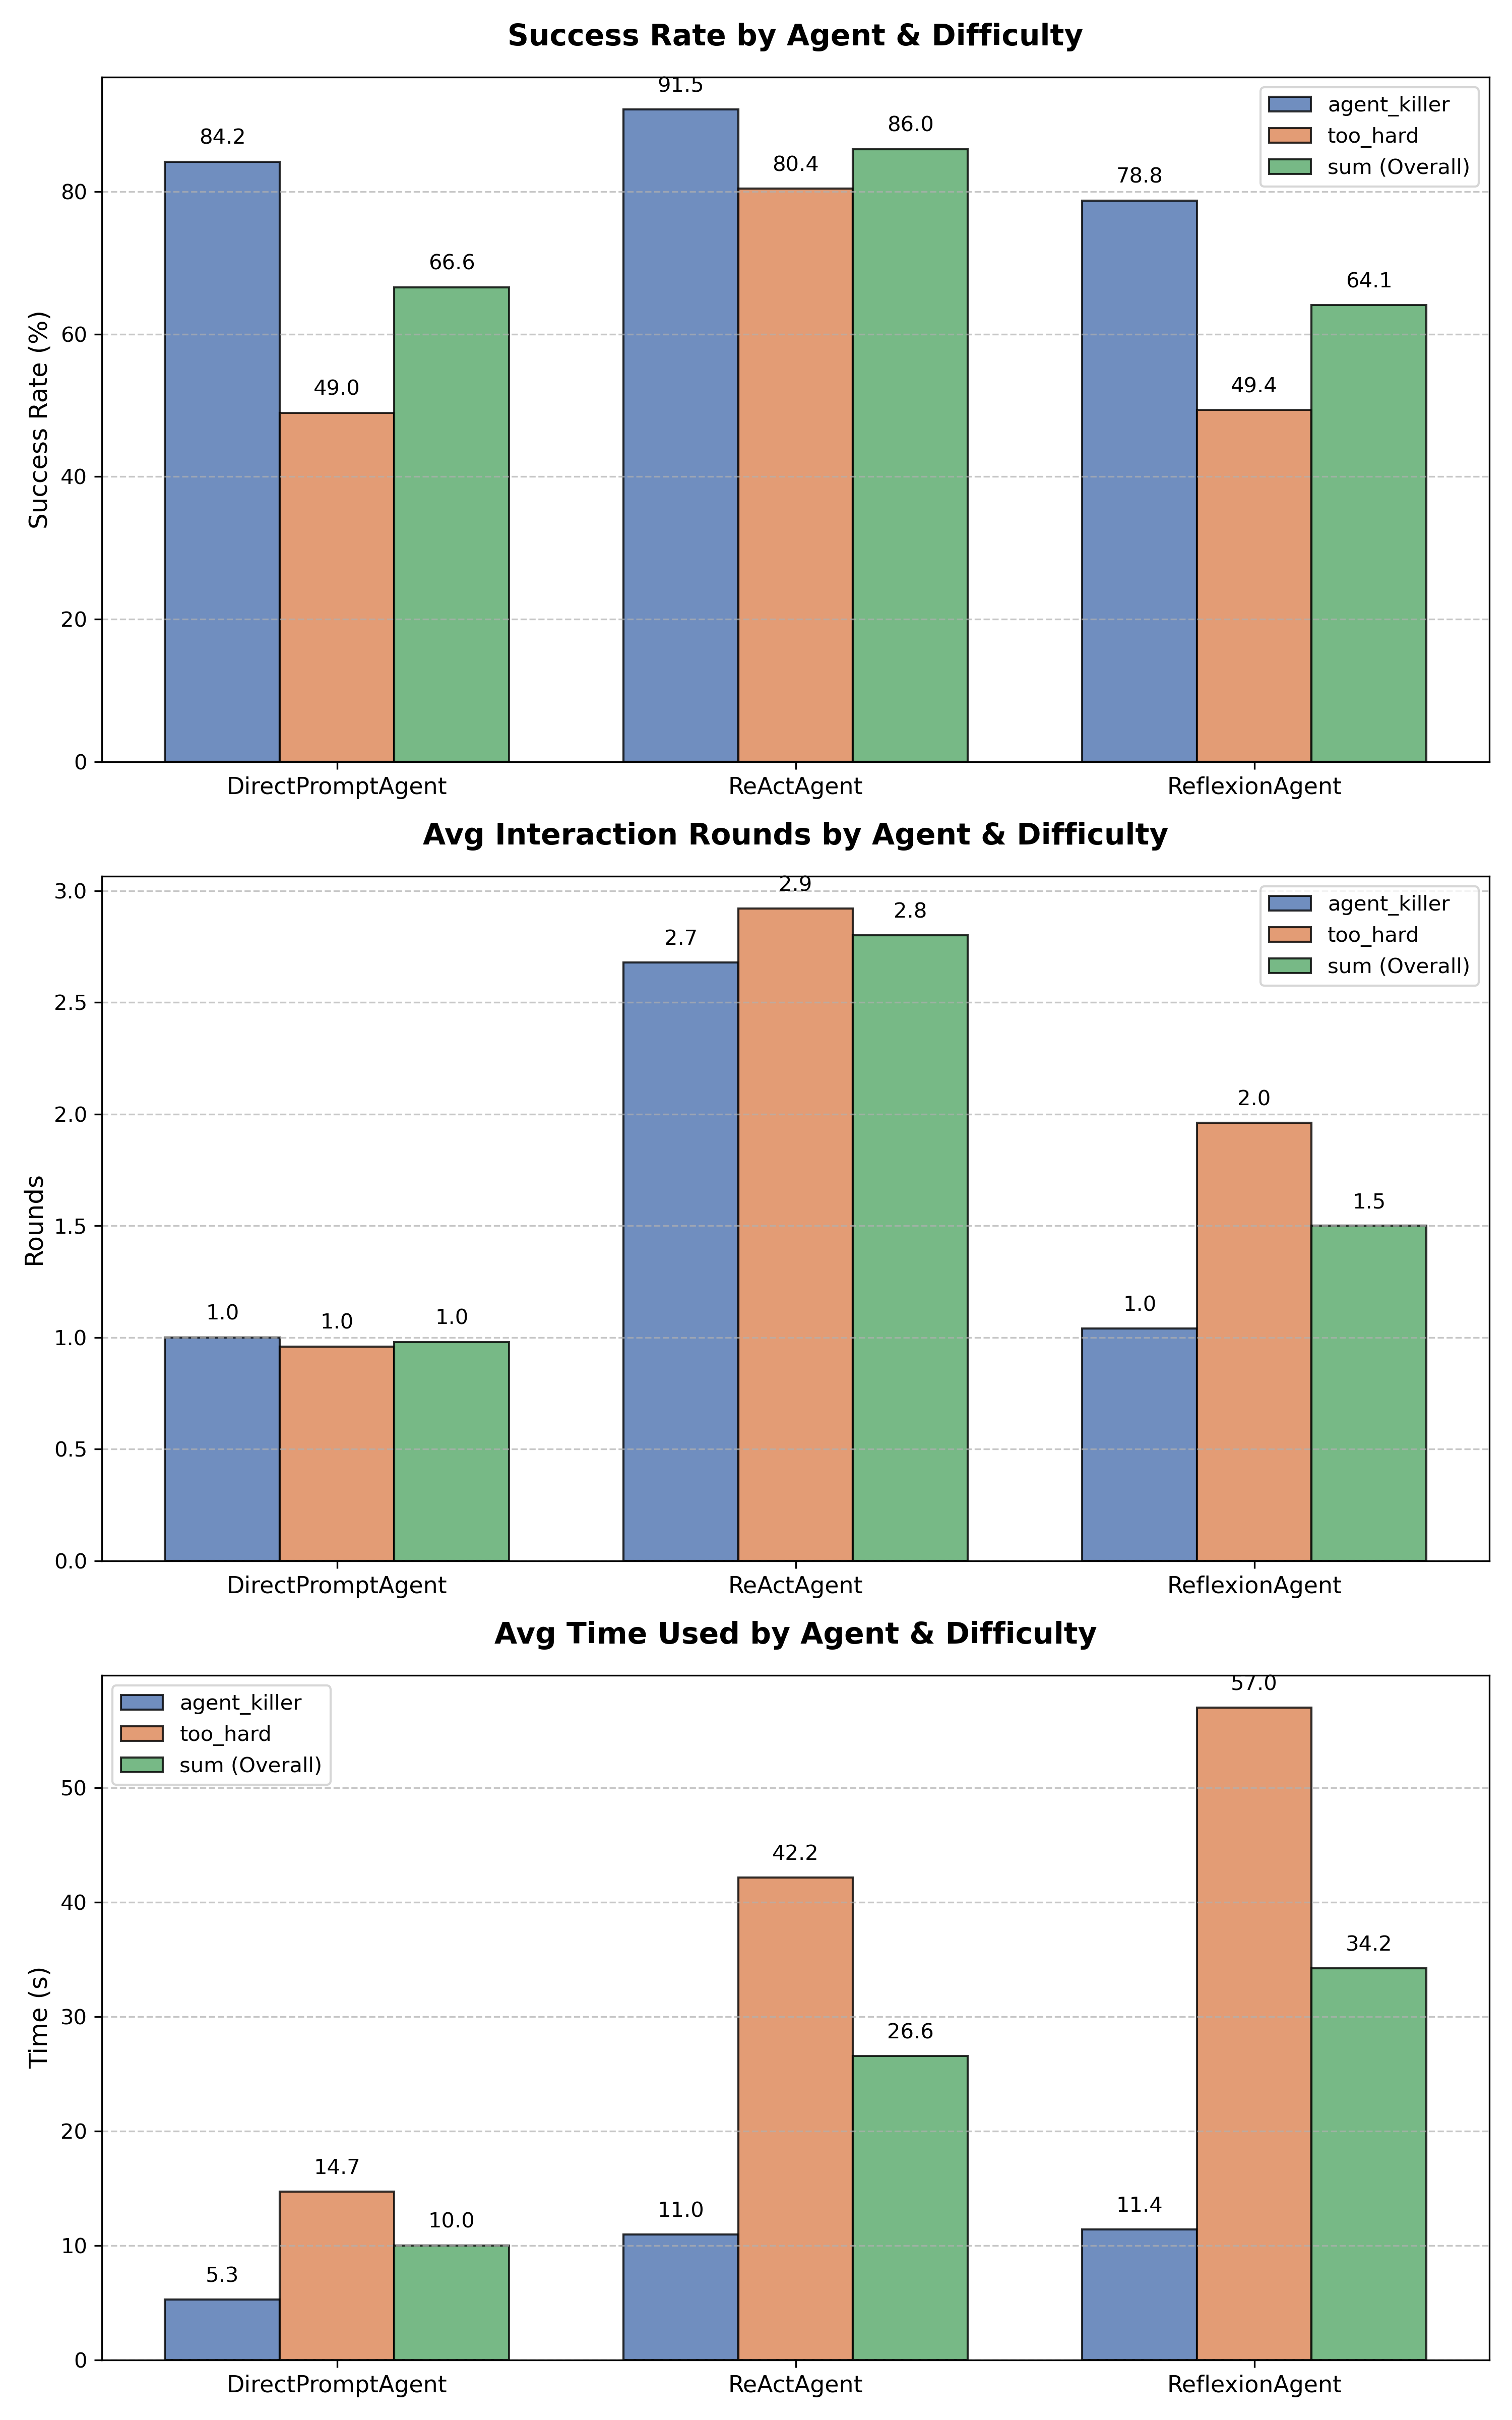
\includegraphics[width=0.8\textwidth]{20260609_182440.png}
    \caption{不同智能体控制流架构评测结果}
    \label{fig:评测结果}
\end{figure}

\end{document}